% Beamer version of the PoC status deck (non-expert audience + expert backup).
% Compile:  pdflatex poc-status-beamer.tex   (run twice for the outline/refs)
\documentclass[aspectratio=169,11pt]{beamer}

\usetheme{Madrid}
\usepackage{tikz}
\usetikzlibrary{arrows.meta,positioning,fit,backgrounds}
\usepackage{booktabs}
\usepackage{xcolor}
\usepackage{pifont}

\definecolor{accent}{HTML}{0B5CAD}
\definecolor{warn}{HTML}{B3261E}
\definecolor{ok}{HTML}{1A7F37}
\definecolor{panel}{HTML}{EEF2F7}

\setbeamercolor{structure}{fg=accent}
\setbeamercolor{frametitle}{bg=accent,fg=white}
\setbeamercolor{title}{bg=accent,fg=white}
\setbeamercolor{subtitle}{fg=accent}
\setbeamertemplate{navigation symbols}{}
\setbeamertemplate{itemize items}[circle]
\setbeamerfont{frametitle}{size=\large}

\newcommand{\good}{\textcolor{ok}{\ding{51}}}
\newcommand{\bad}{\textcolor{warn}{\ding{55}}}

\title[PyTorch $\equiv$ checking with ESBMC]{Proving PyTorch optimizations are correct --- automatically}
\subtitle{Formal equivalence checking of two PyTorch programs with ESBMC}
\date{Proof-of-concept $\cdot$ status update}
\author{Lucas Cordeiro}
\institute{University of Manchester}

\begin{document}

{\setbeamertemplate{footline}{}
\begin{frame}[plain]
  \centering
  \vfill
  \begin{beamercolorbox}[sep=14pt,center,rounded=true,shadow=true,wd=0.92\textwidth]{title}
    \usebeamerfont{title}\inserttitle
  \end{beamercolorbox}
  \vskip0.8em
  {\large\textcolor{accent}{\insertsubtitle}}\par
  \vskip1.6em
  {\large\insertauthor}\par
  \smallskip
  {\small\insertinstitute}\par
  \vskip1em
  {\insertdate}
  \vfill
\end{frame}}

% ---------------------------------------------------------------
\begin{frame}{The problem, in one sentence}
  We constantly \textbf{rewrite} deep-learning code to make it run faster.

  \bigskip
  But how do we \emph{know} the faster version computes the
  \textcolor{warn}{\textbf{same thing}} as the original?

  \bigskip
  \begin{itemize}
    \item A rewrite that is \emph{almost} identical can silently change the results.
    \item Silently wrong math $\rightarrow$ wrong predictions, bugs that are very hard to find.
  \end{itemize}

  \bigskip
  \begin{block}{}
    \centering We want a way to be \textbf{sure}, not hopeful.
  \end{block}
\end{frame}

% ---------------------------------------------------------------
\begin{frame}{Our example: the ``QKV'' step inside every Transformer}
  Attention models --- the engine behind modern AI --- build three things,
  \textbf{Q}, \textbf{K}, \textbf{V}, from the input $X$ using three weight matrices.

  \bigskip
  \textbf{The clear way} (unfused) --- three separate matrix multiplications:
  \[ Q = X\,W_q \qquad K = X\,W_k \qquad V = X\,W_v \]

  \textbf{The fast way} (fused) --- glue the weights together, do \textbf{one} big
  multiply, then split:
  \[ W = [\,W_q \mid W_k \mid W_v\,] \qquad \mathit{QKV} = X\,W \qquad \rightarrow\ \text{split into } Q,K,V \]

  \bigskip
  These \textbf{should} give identical results. The question: do they --- \textcolor{warn}{\emph{always}}?
\end{frame}

% ---------------------------------------------------------------
\begin{frame}{The two programs, side by side}
  \centering
  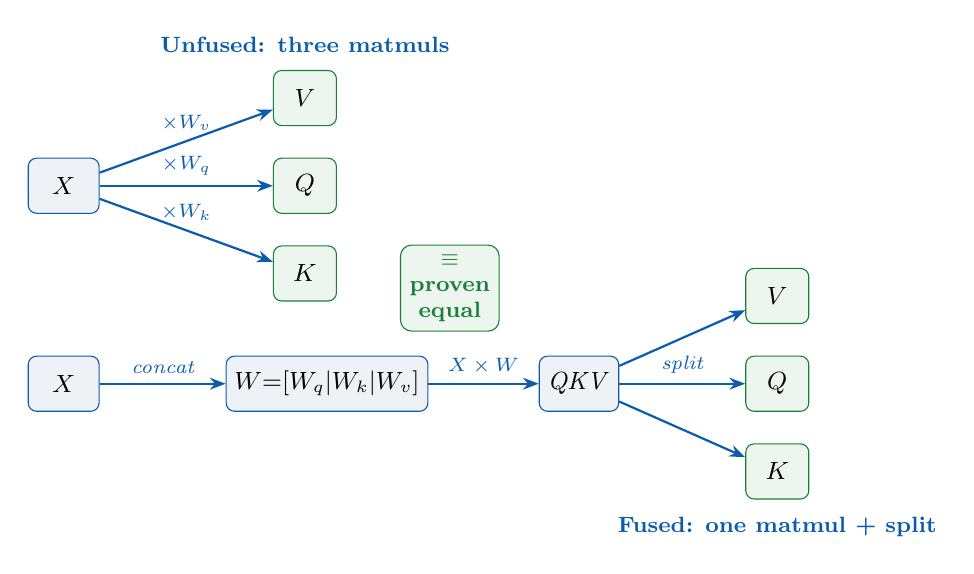
\begin{tikzpicture}[
      font=\small,
      box/.style={rounded corners=3pt,draw=accent,fill=panel,minimum height=7mm,minimum width=9mm,inner sep=3pt},
      res/.style={rounded corners=3pt,draw=ok,fill=ok!8,minimum height=7mm,minimum width=8mm},
      op/.style={midway,above,font=\scriptsize\itshape,text=accent},
      arr/.style={-{Stealth[length=2mm]},thick,accent}]

    \node[box] (xu) {$X$};
    \node[res,right=22mm of xu] (Q) {$Q$};
    \node[res,below=4mm of Q] (K) {$K$};
    \node[res,above=4mm of Q] (V) {$V$};
    \draw[arr] (xu) -- (V) node[op]{$\times W_v$};
    \draw[arr] (xu) -- (Q) node[op]{$\times W_q$};
    \draw[arr] (xu) -- (K) node[op]{$\times W_k$};
    \node[above=1mm of V,text=accent,font=\footnotesize\bfseries] {Unfused: three matmuls};

    \node[box,below=18mm of xu] (xf) {$X$};
    \node[box,right=16mm of xf] (W) {$W{=}[W_q|W_k|W_v]$};
    \node[box,right=14mm of W] (QKV) {$\mathit{QKV}$};
    \node[res,right=16mm of QKV] (Qf) {$Q$};
    \node[res,below=4mm of Qf] (Kf) {$K$};
    \node[res,above=4mm of Qf] (Vf) {$V$};
    \draw[arr] (xf) -- (W) node[op]{concat};
    \draw[arr] (W) -- (QKV) node[op]{$X\times W$};
    \draw[arr] (QKV) -- (Vf) node[op,font=\tiny\itshape]{};
    \draw[arr] (QKV) -- (Qf) node[op]{split};
    \draw[arr] (QKV) -- (Kf) node[op,font=\tiny\itshape]{};
    \node[below=1mm of Kf,text=accent,font=\footnotesize\bfseries] {Fused: one matmul {+} split};

    \node[draw=ok,rounded corners,fill=ok!8,text=ok,font=\footnotesize\bfseries,
          right=8mm of Q,yshift=-13mm,align=center] (eq)
      {$\equiv$ \\ proven\\ equal};
  \end{tikzpicture}

  \medskip
  {\small ESBMC proves these two produce \textbf{the same result for every input we model}.}
\end{frame}

% ---------------------------------------------------------------
\begin{frame}{How we check today: we test}
  We run the program on a \textbf{handful of example inputs} and compare.

  \bigskip
  \centering{\Large \emph{Like tasting a few spoonfuls of soup and hoping the whole pot is fine.}}

  \bigskip
  \begin{itemize}
    \item Testing only covers the inputs you happened to try.
    \item A bug hiding in some other input is simply \textbf{missed}.
    \item \textcolor{warn}{\textbf{Passing tests $\neq$ correct.}}
  \end{itemize}
\end{frame}

% ---------------------------------------------------------------
\begin{frame}{What we actually want: a proof, not a sample}
  Instead of trying a few inputs, check \textbf{every input we model --- all at once} --- mathematically.

  \bigskip
  Two possible outcomes:
  \begin{itemize}
    \item \good\ \textbf{PROVEN equal} --- guaranteed identical for \emph{every} input in the model.
    \item \bad\ \textbf{Counterexample} --- one specific input where they differ, handed straight to you.
  \end{itemize}

  \bigskip
  Either way, you learn something \textbf{certain}.
\end{frame}

% ---------------------------------------------------------------
\begin{frame}{The tool: ESBMC}
  \textbf{ESBMC} is an automated \emph{model checker}.

  \bigskip
  \begin{enumerate}
    \item It \textbf{reads the program} and turns the question \emph{``are these two always
      equal?''} into one giant logic puzzle.
    \item An automated \textbf{solver} then either finds an input that breaks it, or proves
      that \textbf{no such input exists} (within the model).
  \end{enumerate}

  \bigskip
  \begin{block}{}
    \centering \textbf{Fully automated} once the program is encoded --- you write \emph{no} proofs by hand.
  \end{block}
\end{frame}

% ---------------------------------------------------------------
\begin{frame}{The trick that turns a test into a proof}
  \centering
  \begin{tabular}{@{}p{0.42\textwidth} p{0.44\textwidth}@{}}
    \toprule
    \textbf{Ordinary test} & \textbf{Our verification} \\
    \midrule
    one \textbf{random} tensor \texttt{torch.randn(\dots)} & a \textbf{symbolic} tensor = \emph{any} numbers (bounded) \\[4pt]
    checks that one case & checks the \textbf{whole modelled range at once} \\[4pt]
    ``looks fine'' & a \textbf{guarantee --- within the model} \\
    \bottomrule
  \end{tabular}

  \bigskip
  We assert \texttt{unfused == fused}, feed it \emph{any} input in range, and let ESBMC settle it.

  \medskip
  {\footnotesize Inputs are bounded to a finite range to exclude ``not-a-number''. ($\rightarrow$ Assumptions, backup.)}
\end{frame}

% ---------------------------------------------------------------
\begin{frame}{Result: the example is PROVEN correct}
  \begin{itemize}
    \item \good\ Proven equal for \textbf{all inputs we model} --- and \textbf{bit-for-bit exact}
      (IEEE-754), not a ``close enough'' tolerance.
    \item \good\ Done \textbf{two ways}: a plain-math encoding \emph{and} the real
      \texttt{torch.mm} {+} \texttt{torch.allclose}.
    \item \good\ When we \textbf{deliberately break it} (swap two columns), ESBMC
      \textbf{catches it} and shows the exact failing input.
  \end{itemize}

  \bigskip
  {\footnotesize What ``modelled'' means (fixed sizes, bounded inputs) $\rightarrow$ \textbf{Assumptions \& Scope}, backup.}
\end{frame}

% ---------------------------------------------------------------
\begin{frame}{What the suite covers (and what it doesn't --- yet)}
  \textbf{6 / 6} checks behave as expected --- small \emph{on purpose}: it is breadth, not scale.

  \medskip
  \begin{tabular}{@{}ll@{}}
    \toprule
    \textbf{Dimension} & \textbf{Coverage} \\
    \midrule
    Problem classes & QKV projection $\cdot$ bias-fused linear ($X\,W + b$) \\
    Encodings & plain-math \textbf{and} torch-native (\texttt{torch.mm} / \texttt{allclose}) \\
    Check type & a \textbf{proof} (clean $\Rightarrow$ \good) \textbf{and} a \textbf{refutation} (bug $\Rightarrow$ \bad\ {+} counterexample) \\
    \bottomrule
  \end{tabular}

  \medskip
  {\footnotesize Every case is double-checked: we prove the correct version \emph{and} confirm a broken one is
  caught. \textbf{Early-stage PoC} --- small fixed sizes for now (see Performance, backup).}
\end{frame}

% ---------------------------------------------------------------
\begin{frame}{Why this matters}
  \begin{itemize}
    \item \textbf{All modelled inputs}, not a few $\rightarrow$ no hidden corner cases within the model.
    \item \textbf{Exact} $\rightarrow$ catches tiny numerical drift that testing would wave through.
    \item \textbf{Automated} $\rightarrow$ no hand-written proofs.
    \item \textbf{Actionable failures} $\rightarrow$ it gives you the precise input that breaks things.
  \end{itemize}

  \bigskip
  \begin{block}{}
    Concretely: \textbf{detect incorrect optimizations early} and \textbf{validate fusion / compiler
    transformations} \emph{before} they ship.
  \end{block}
\end{frame}

% ---------------------------------------------------------------
\begin{frame}{A bonus: we made the tool itself stronger}
  Real PyTorch-style code pushed ESBMC into territory it could not yet handle ---
  so we \textbf{added what was missing} (4 contributions merged upstream):

  \bigskip
  \begin{itemize}
    \item A \textbf{\texttt{torch} operational model} --- \texttt{mm}, \texttt{matmul}, \texttt{cat},
      \texttt{split}, \texttt{allclose}.
    \item Fixes so \textbf{matrix math over nested lists works} --- values/types survive function
      returns and copies.
    \item A \textbf{floating-point element-type fix} for matrices built by comprehension
      (we found, root-caused, and fixed it).
  \end{itemize}

  \bigskip
  {\footnotesize Result: PyTorch-style code is now verifiable in ESBMC \textbf{at all} --- reusable by anyone.}
\end{frame}

% ---------------------------------------------------------------
\begin{frame}{Where we are $\cdot$ what's next}
  \begin{itemize}
    \item \good\ Motivating \textbf{QKV} example \textbf{fully supported} (two encodings, exact proof).
    \item \good\ Extended to a \textbf{second} class: bias-fused linear ($X\,W + b$).
    \item $\rightarrow$ \textbf{Bigger matrices} and fully native fuse/split --- gated on \textbf{one}
      performance improvement upstream (see Performance, backup).
  \end{itemize}
\end{frame}

% ---------------------------------------------------------------
{\setbeamertemplate{footline}{}
\begin{frame}[plain]
  \centering
  \vfill
  {\Large\textcolor{accent}{\textbf{Takeaway}}}

  \bigskip
  We can \textbf{prove} --- automatically, for \textbf{every modelled input} ---
  that a fast PyTorch rewrite computes \textbf{exactly} the same result as the original.

  \bigskip
  \emph{Testing samples. This proves --- and when it can't, it hands you the bug.}

  \bigskip
  \textbf{Use it to gate fusions and compiler rewrites before they ship.}
  \vfill
\end{frame}}

% =============================================================
\appendix

{\setbeamertemplate{footline}{}
\begin{frame}[plain]
  \centering\vfill
  {\Large\textcolor{accent}{\textbf{Backup slides}}}

  \medskip
  {\normalsize Assumptions $\cdot$ Under the hood $\cdot$ Performance}
  \vfill
\end{frame}}

% ---------------------------------------------------------------
\begin{frame}{Backup: Assumptions \& Scope}
  \textbf{What we prove}
  \begin{itemize}
    \item Equivalence of the two programs \emph{as written}, for \textbf{all inputs in the modelled range}.
    \item Floating-point modelled \textbf{exactly} (IEEE-754, bit-precise) --- not real arithmetic,
      not a hand-waved tolerance.
  \end{itemize}

  \textbf{What we model / bound}
  \begin{itemize}
    \item \textbf{Fixed tensor sizes} (bounded model checking; concrete, e.g. $S{=}1, D{=}2, H{=}1$).
    \item \textbf{Inputs bounded} to a finite range, which excludes \texttt{NaN}/\texttt{Inf}.
  \end{itemize}

  \textbf{What we do \emph{not} claim:} arbitrary/symbolic sizes $\cdot$ performance equivalence
  $\cdot$ behaviour outside the bounds.
\end{frame}

% ---------------------------------------------------------------
\begin{frame}[fragile]{Backup: under the hood --- how verification works}
  \begin{enumerate}
    \item ESBMC \textbf{unrolls} the program (fixed sizes $\Rightarrow$ finite) and turns each
      \texttt{assert} into a \textbf{verification condition}.
    \item Tensors are modelled as lists of \textbf{IEEE-754 floats}; \texttt{torch.mm} /
      \texttt{torch.allclose} have operational models.
    \item The condition is essentially: \emph{for all bounded inputs,} \texttt{fused[i][j] == unfused[i][j]}.
    \item An \textbf{SMT solver} (Bitwuzla / Z3) decides it: \textbf{UNSAT $\Rightarrow$ proved};
      \textbf{SAT $\Rightarrow$ counterexample}.
  \end{enumerate}

  \begin{semiverbatim}\footnotesize
X, Wq, Wk, Wv = symbolic, bounded        \# any numbers in range
assert torch.allclose(unfused, fused)    \# -> one SMT formula over FP
  \end{semiverbatim}
\end{frame}

% ---------------------------------------------------------------
\begin{frame}{Backup: performance \& current limits}
  \begin{center}
  \begin{tabular}{@{}ll@{}}
    \toprule
    \textbf{Check} & \textbf{Time} (Bitwuzla, macOS arm64) \\
    \midrule
    scalar QKV proof & $\sim$11 s \\
    torch-native QKV proof & $\sim$110 s \\
    refuting a broken variant & 31--292 s \\
    \bottomrule
  \end{tabular}
  \end{center}

  \begin{itemize}
    \item Cost grows quickly with tensor size (more multiply-adds $\rightarrow$ a bigger FP formula).
    \item \texttt{torch.cat} / \texttt{torch.split} are modelled but \textbf{unwinding-heavy}
      (a $1{\times}1{\times}3$ \texttt{cat}+\texttt{split} $\approx$ 2.5 min) $\rightarrow$ we fuse/split
      by manual indexing for now.
    \item \textbf{Scaling to realistic sizes is the main open bottleneck} (tracked upstream).
  \end{itemize}
\end{frame}

\end{document}
